\chapter{Evaluation}
\label{chapter:evaluation}

Kata Containers hardens the security of containerized environment by adding the extra layer of security with the micro-VM. The architectural change and new components of the environment enable the additional security features. However, these components, such as the micro-VM and hypervisor, come with a possible price of degraded performance and computational overhead. Previous work, such as \cite{EverartsdeVelp2020} and \cite{Kumar2020} have examined the performance when compared Kata Containers against the native runtime runC, the most common OCI-compliant runtime. In these two papers, Kata Containers architecture design results in a performance decrease in disk and memory-based I/O throughput and overhead in memory and CPU utilization. However, the results in these papers are highly dependant on the underlying test environment. Furthermore, these tests do not consider the latest development and performance optimization of Kata Containers' performance. This paper evaluates the system performance in an environment simulating a telco Edge Cloud architecture and regular workload by performing I/O tests for disk and memory-based volumes.

\section{Test architecture}
\label{section:test_architecture}

Telco applications are relying on high-performing and optimized computing. The ever-more increasing performance requirements from users add a great demand on the underlying infrastructure. Software and hardware-based architectural changes to the Edge Cloud environment need to be carefully evaluated before implementing them into the production. Otherwise, it might stall the performance and significantly decrease the performance for mobile network users.

The test environment, visualized in Figure \ref{fig:TestArchitectureCluster}, is a simple single-node cluster with one container. The main focus of the tests is to evaluate the impact of Kata Containers and the choice of the hypervisor to I/O operations throughput and latency on various storage methods, such as PV, emptyDir, and hostPath. Table \ref{table:TestMatrix} describes the full test combination matrix. The test cluster is hosted on K3s \cite{K3s} version 1.17.3, a lightweight version of Kubernetes supporting the identical API. K3s is Kubernetes distribution built for IoT and edge computing with a lower footprint on memory and disk usage. K3s uses containerd as a native container runtime engine. Due to compatibility issues, Kata Containers uses version 1.12.0, which benefits from the simplified Kata Shim V2 \cite{KataContainersArchitecture} architecture described in Figure \ref{fig:KataContainersArchitecture}.

\begin{figure}[ht]
  \begin{center}
    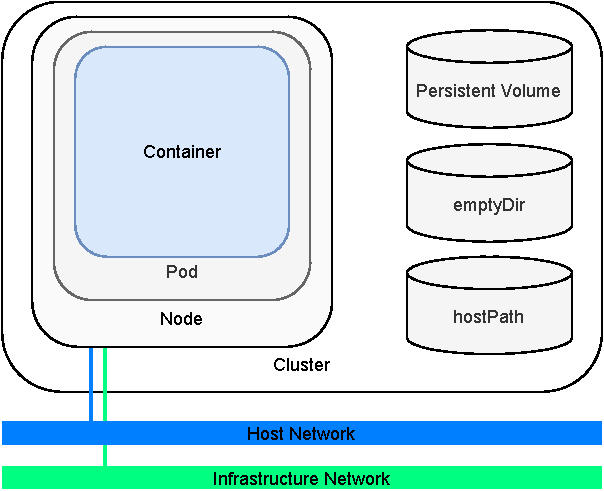
\includegraphics[width=12cm]{images/TestArchitectureClusterSimple.pdf}
    \caption{Kubernetes test cluster overview}
    \label{fig:TestArchitectureCluster}
  \end{center}
\end{figure}

\section{Methodology}

The tests of this thesis aim to measure the possible performance degradation of I/O operations, such as bandwidth and completion latency. A dedicated server hosts the test environment, and the underlying hardware is built and tailored to support Edge and Far Edge Cloud deployments. The server includes an Intel Xeon 6212U CPU with 24 cores and 48 threads with x86 architecture at 2.40 GHz clock-speed and 192 GB of DDR4 memory at 2933 MHz clock speed, which is shared to the cluster.

The host runs CentOS 8 and uses Linux kernel version 4.18.0-240.22.1, affecting mostly bare-metal and runC environments. In Kata Containers, CLH and QEMU with VirtioFS use version 5.6.0, whereas QEMU uses a slightly older kernel version of 5.4.60. The difference in kernel versions might affect the performance results due to optimization in resource usage and I/O operations. The server uses Intel's SSD \cite{IntelSSD} for disk-based I/O operations. This disk's theoretical maximum bandwidth for sequential read operations is up to 560 MB/s and 510 MB/s for write operations.

The performance tests run with Fio \cite{FIO}, an I/O performance tester intending to simulate a variety of I/O workloads without resorting to writing tailored test cases repeatedly. Fio supports various test configurations such as multiple threads, block sizes, I/O sizes, and I/O patterns. In this thesis, the tests are time-based, where each test runs for 30 seconds. The file size of each writable file is 2 GB. The Fio configuration file, also known as the job file, is described in Appendix \ref{appendix:fio_jobfile}. Each test is repeated three times, and averaging the results. Table \ref{table:TestMatrix} describes the test combination matrix. In the tests, each possible combination is sampled, resulting in 1428 different test scenarios. To be noted, bare-metal tests allow only I/O to a disk volume. Kubernetes hosted tests, runC and Kata Containers, leverage all disk and memory-based volumes. The span of the disk for bare-metal volume is the full 480 GB, whereas Kubernetes hosted volumes can be split into smaller units, resulting in a narrower span for read and write operations. This variance in span highly affects the efficiency of seek operations.

\begin{table}[ht]
\centering
\caption{Test combinations matrix}
\vspace{\baselineskip}
\begin{tabular}{| c | c | c | c | c |}
\hline
\textbf{Runtime} & \textbf{Jobs} & \textbf{Block size} & \textbf{I/O pattern} & \textbf{I/O device} \\ 
\hline
Bare-metal & 1 & 512 & read & emptyDir (memory) \\
\hline
runC & 2 & 1024 & write & emptyDir (disk) \\ 
\hline
CLH & 3 & 2048 & randread & local (PV) \\
\hline
QEMU & & 4096 & randwrite & hostPath \\
\hline
QEMU VirtioFS & & 8192 & & \\
\hline
& & 32768 & & \\
\hline
& & 65536 & & \\
\hline
\end{tabular}
\label{table:TestMatrix}
\end{table}

The test matrix consists of five columns: runtime, jobs, block size, I/O pattern, and I/O device, the runtime of the tests refers to the container runtime or hypervisor. In the case of bare-metal, the test is run directly on the host without containerization. In bare-metal test runs, the performance test is launched with CPU affinity to an isolated CPU with taskset \cite{taskset} command. Jobs refer to the number of concurrent clones. Each clone of the job is spawned as an independent thread or process. Block size is the size in bytes for I/O units applying for reads and writes. I/O pattern has sequential and random pattern reads and writes. I/O type of the test is buffered, as configured in the Fio job file. I/O device refers to the storage volumes used for the test destination. EmptyDir is created within the container of these storage volumes, whereas the host maintains local Persistent Volume and hostPath.

Fio test suite is wrapped inside a Docker image with a Linux OS Alpine \cite{Alpine}, which aims to deliver general-purpose Linux with security, simplicity, and resource efficiency. The tests containers are deployed into the test cluster with Helm \cite{Helm}, a package manager for Kubernetes helping with the deployment of applications. These applications are deployed in Kubernetes pods as Guaranteed Quality-of-Service \cite{QOSKubernetes} with two CPUs and 18 GB of memory to support the tests. However, each Kata Containers' VM and runC container gets assigned only with one CPU. This restriction allows better comparison tests to bare-metal tests run on an isolated single CPU environment. The Guaranteed Quality-of-Service prevents Kubernetes from scheduling other containers for the same core. However, this does not guarantee that the underlying system would not assign low-level system tasks on the same core. The comparable isolation to taskset, as in bare-metal, could only be achieved with core isolation plugins, such as Nokia's CPU Pooler, limiting the absolute comparison of results described in the next section.

\section{Results}

Previous work \cite{EverartsdeVelp2020}\cite{Kumar2020}\cite{StackHPCKata}\cite{Randazzo2019} on measuring Kata Containers' performance resulted in highly unified performance between bare-metal and runC. In read and write tests, runC slightly outperformed the tested Kata Containers setups with faster throughput and lower resource usage. However, the results of these papers varied due to the diversity in underlying infrastructure and the difference in test frameworks. None of these researches tested the whole spectrum of hypervisors and various storage options offered in the Kubernetes environment.

The hypervisor of Kata Containers adds its resource and latency overhead to the performance. The focal point of I/O tests is to evaluate the performance of Kata Containers with various hypervisors against the runC runtime and determine the inherent performance metrics of each hypervisor and evaluate storage volume performance. As described in Table \ref{table:TestMatrix}, the test includes three different Kata Containers' hypervisors: CLH, QEMU, and QEMU with VirtioFS. Secure container runtimes leveraging micro-VM include hypervisor to the stack. This hypervisor includes its cache, giving a false impression of superior performance compared to bare-metal and runC. The caching feature restricts the possible comparison of bare-metal's and runC's performance evaluation to secure runtimes in read operations for all disk-based storage volumes.

Kubernetes offers multiple storage options for various deployments, and each of these options provides slightly different performance and features. The tests include four storage options suitable for the telco environment: disk and memory-based emptyDir, hostPath as Persistent Volume, and hostPath. The second key point of the tests is to evaluate these storage methods concerning block sizes between 512 bytes and 64 KBs and concurrent jobs from one to three. It is essential to make the distinction of evaluating the best option for non-persistent and persistent volumes.

Tests to evaluate the performance are run individually to minimize interference, and the final results are averaged out of three test runs. Fio test suite provides a comprehensive catalog of parameters as test results. These test results are divided into two categories, which are bandwidth and completion latency. Bandwidth, or I/O throughput in megabytes per second, is the sum of block size multiplied by the number of I/O operations per second. Bare-metal test results work as a benchmark of the best-case scenario for disk-based volumes. Completion latency describes the completion time in milliseconds for key percentiles such as 50\% and 99\%. 

\subsection{Bandwidth}

Figure \ref{fig:ResultsVolumeByRTC4096-1} visualizes the effect of runtime class for reading or write bandwidth for the four storage volumes. Bare-metal is not comparable with memory-based emptyDir, due to significantly different techniques used, and thus it is not plotted for emptyDir on memory. Memory-based emptyDir achieves the highest bandwidth as it reaches over 2 GB/s with sequential read and over 1.9 GB/s with sequential write for all runtimes. The performance slightly degrades for random pattern read and write operations but achieves over 1.5 GB/s performance for all runtimes. Hypervisor-based runtimes seem to perform highly alike, with only minor differences between them. Based on the acquired test results in Figure \ref{fig:ResultsPVByBS-1} with PV as volume and one concurrent job, CLH outperforms QEMU-based runtime classes in tests with smaller block sizes, 512 to 8192. The trends flip for tests with block sizes 32768 and 65536. Due to the caching, bare-metal and runC are not comparable against Kata Container runtimes in reading operations.

Hypervisor caching affects the confidence in the test results highly for reading operations, especially random pattern read. When fetching data from a storage volume, the system first checks the memory-based cache for the request data. If it is found, the seek on a storage volume is skipped. As the size of each job file in Fio was relatively small, the hit probability of the requested block being cache is high, which skews the results in favor of Kata Containers runtimes. This effect of caching is visible in Figure \ref{fig:ResultsVolumeByRTC4096-1} where Kata Containers runtimes outperform bare-metal and runC in all disk-based sequential, and random pattern read tests by a clear margin. The same skew is also visible in Figure \ref{fig:ResultsHPClatByRTC4096-2}, where completion latency is lower for hostPath read operations.

\begin{figure}[ht]
  \begin{center}
    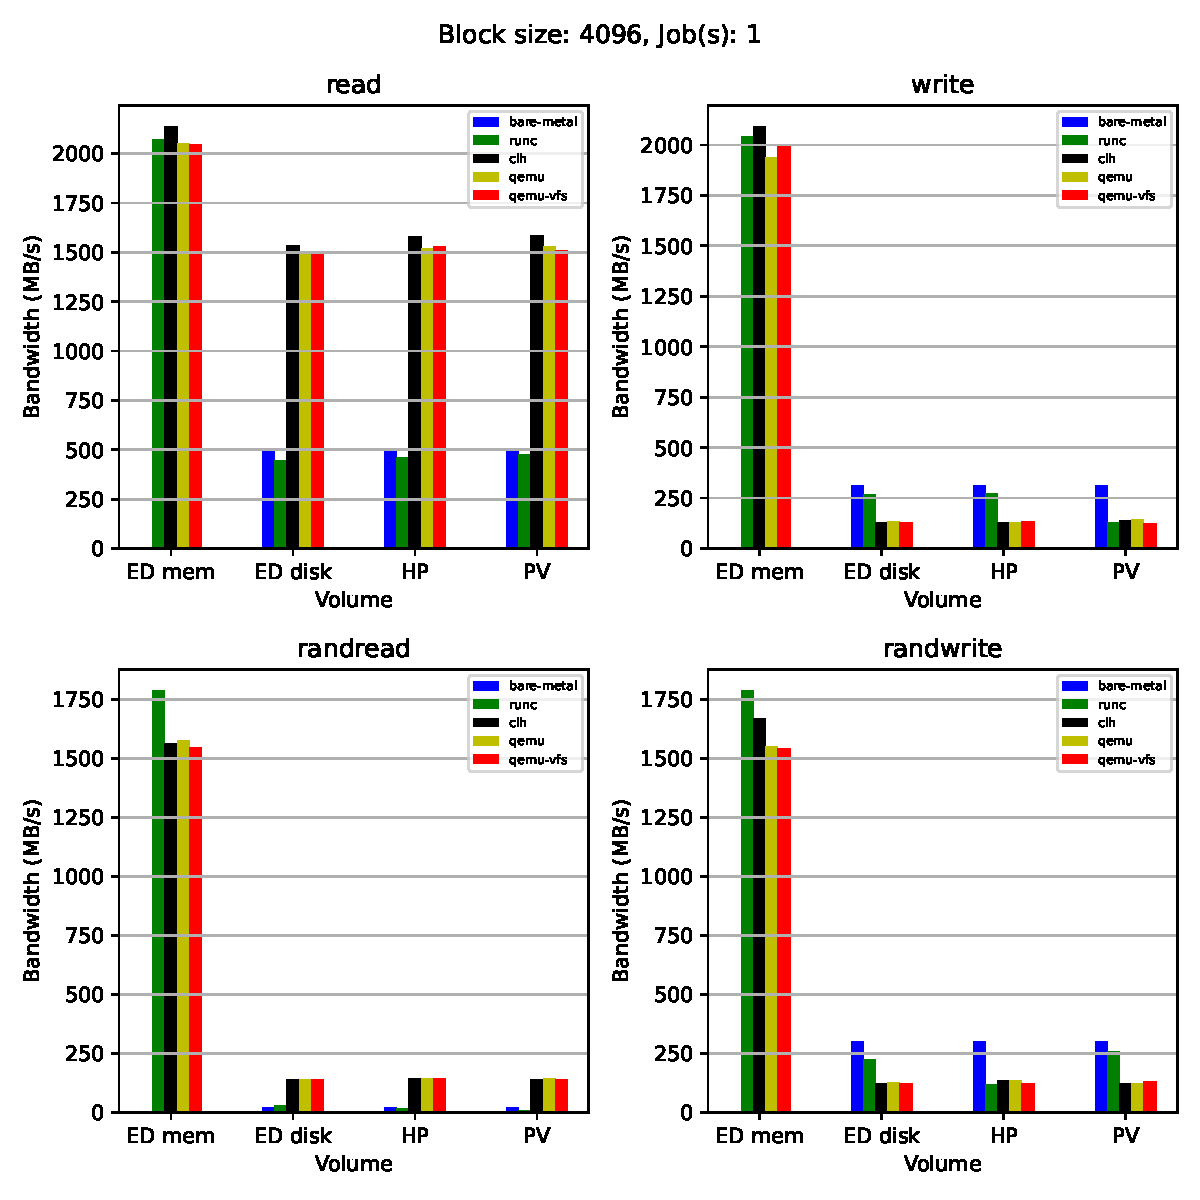
\includegraphics[width=12cm]{results/subplot_bw_by_volume_with_bare(4096,1).pdf}
    \caption{Comparison of volume performance by runtime classes for 4096 bytes block size and one job}
    \label{fig:ResultsVolumeByRTC4096-1}
  \end{center}
\end{figure}

For write operations in Figure \ref{fig:ResultsVolumeByRTC4096-1}, runC averages 224 MB/s on sequential and 201 MB/s on random patterns with disk-based volumes. In contrast, Kata Containers averages 131-135 MB/s on sequential and 127-129 MB/s on random pattern write operations. The proportional drop in performance is significant, resulting in around 36-40\% drop in the bandwidth. This drop in performance is radical compared to memory-based emptyDir, which suggests leveraging memory for as much as possible. Kata Containers runtimes perform on the same level, with no clear differences in the bandwidth across them. The performance of disk-based volumes is highly correlated, with no difference in performance for persistent and non-persistent volumes for Kata Containers runtimes.
    
Figure \ref{fig:ResultsPVByBS-1} visualizes the effect of block size on the bandwidth on Persistent Volume. The caching affects Kata Containers' runtimes results, interfered with by reading and writing operations over-performing the maximum disk bandwidth. Also, in this test, the bandwidth performance of Kata Containers runtimes makes no apparent difference.

\begin{figure}[ht]
  \begin{center}
    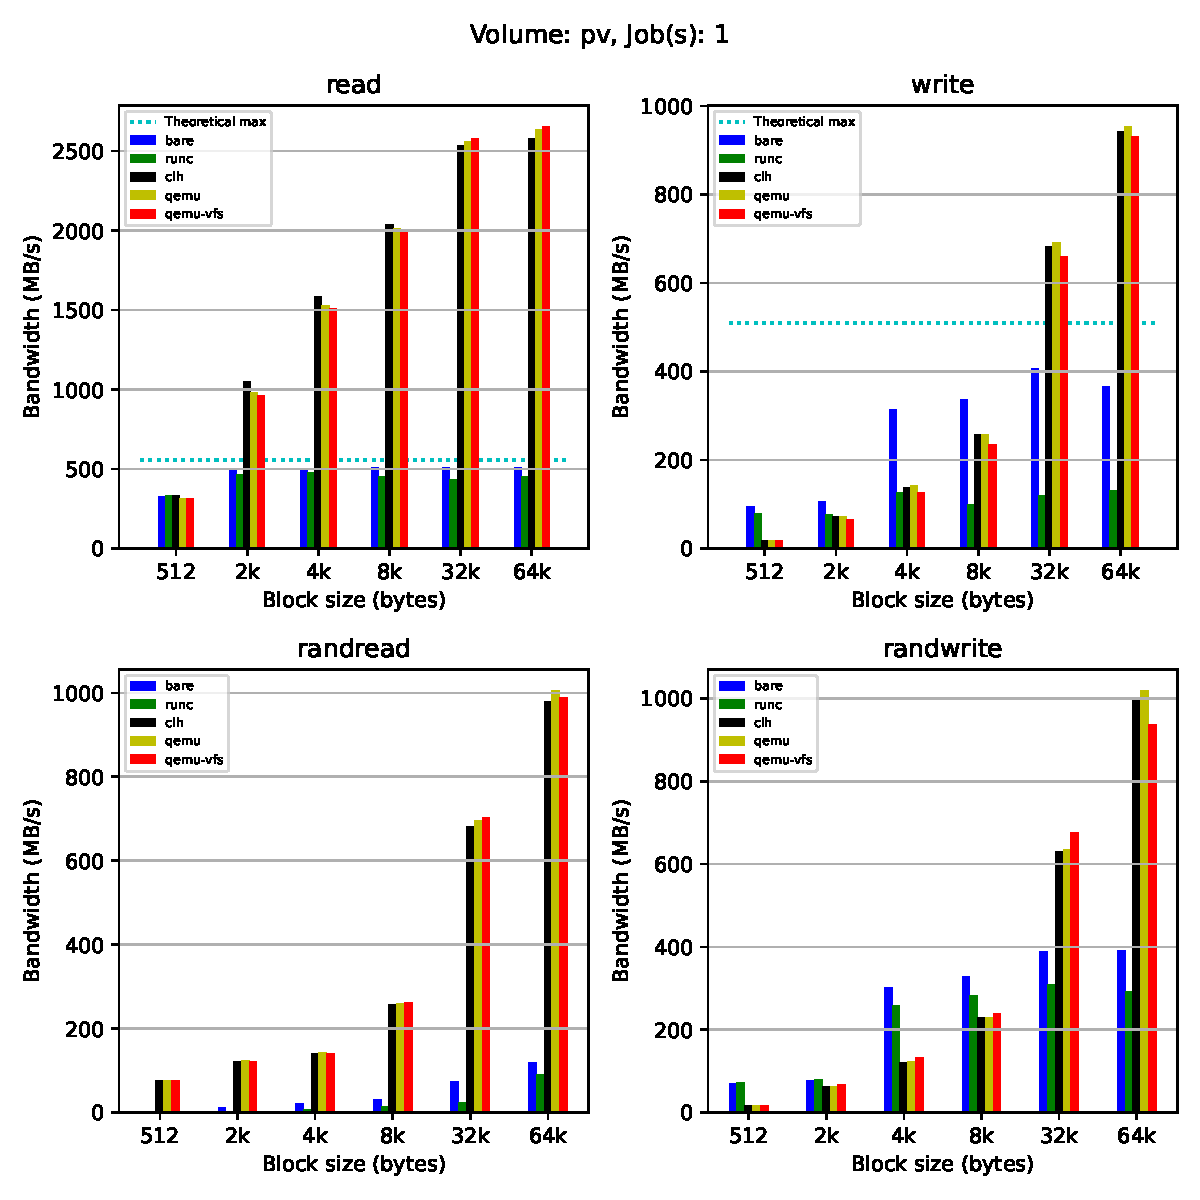
\includegraphics[width=12cm]{results/subplot_bw_by_bs_with_bare(pv,1).pdf}
    \caption{Bandwidth comparison for Persistent Volume by block sizes for all runtime classes with one job}
    \label{fig:ResultsPVByBS-1}
  \end{center}
\end{figure}

Memory-based volume outperforms disk-based storage volumes for two reasons. First, the bandwidth of memory is significantly higher due to architectural differences. Meanwhile, the latency of operations drops close to real-time. Memory-based emptyDir volume is at most 50\% of the memory assigned to the VM \cite{VolumesKubernetes}. The VMs are assigned with 16 GB of memory; thus, the memory-based emptyDir allows at most 8 GB volume. This storage allocation is slightly smaller concerning disk-based storage mediums ED disk and PV. Test environments orchestrated by Kubernetes are launched with a Persistent Volume Claim of 10 GBs. In contrast, bare-metal read operations use the whole 100\% span of the 480 GB SSD \cite{IntelSSD} highly dropping the performance as the operations span across a broader range in the SSD. The smaller volume size allows random seeks to hit with higher confidence, thus increasing the bandwidth of random read operations.

\subsection{Completion latency}

Figures \ref{fig:ResultsEDMEMClatByRTC4096-2} and \ref{fig:ResultsHPClatByRTC4096-2} visualize the performance for completion latency for emptyDir on memory and hostPath volumes by all runtime classes with 4096 byte block sizes and two concurrent jobs. The plots include latencies for 50th and 99th percentile completion of the tasks. Appendix \ref{table:ResultsEDMEMClatByRTC4096-2} includes more detailed results for Figure \ref{fig:ResultsEDMEMClatByRTC4096-2}. RunC narrowly outperforms VM-based runtime classes in memory-based emptyDir by a 3 to 10 ms margin. This difference indicates the overhead from the micro-VM to memory-based operations. The tail for completion of last percentiles in memory-based volume operations is considerably larger for Kata Containers in comparison to runC.

Figure \ref{fig:ResultsHPClatByRTC4096-2} includes also bare-metal for comparison in hostPath volume. Overall, bare-metal and runC performs the best with the lowest latencies. The performance difference between Kata Containers and runC grows larger for disk-based volumes. Read operations are skewed in favor of micro-VMs due to the caching. Surprisingly, the tail for bare-metal and runC grows along with the last five percentiles in reading operations.

Write operations are less affected by the caching and can be more reliably compared. Bare-metal and runC perform with highly similar results with 4 kB block size and hostPath volume. In Figure \ref{fig:ResultsHPClatByRTC4096-2} the first sequential write task is completed with around 17-19 ms overhead, and the 50th percentile stands at 18-24 ms. RunC adds only 2 ms or 7-8.5\% increment to the bare-metal benchmark for the 99th percentile. Respectively, Kata Containers' runtimes complete the first task at around 200 ms. 50th and 99th percentile are completed at 218-231 ms and 258-272 ms, which is over 200 ms addition.

\begin{figure}[ht]
  \begin{center}
    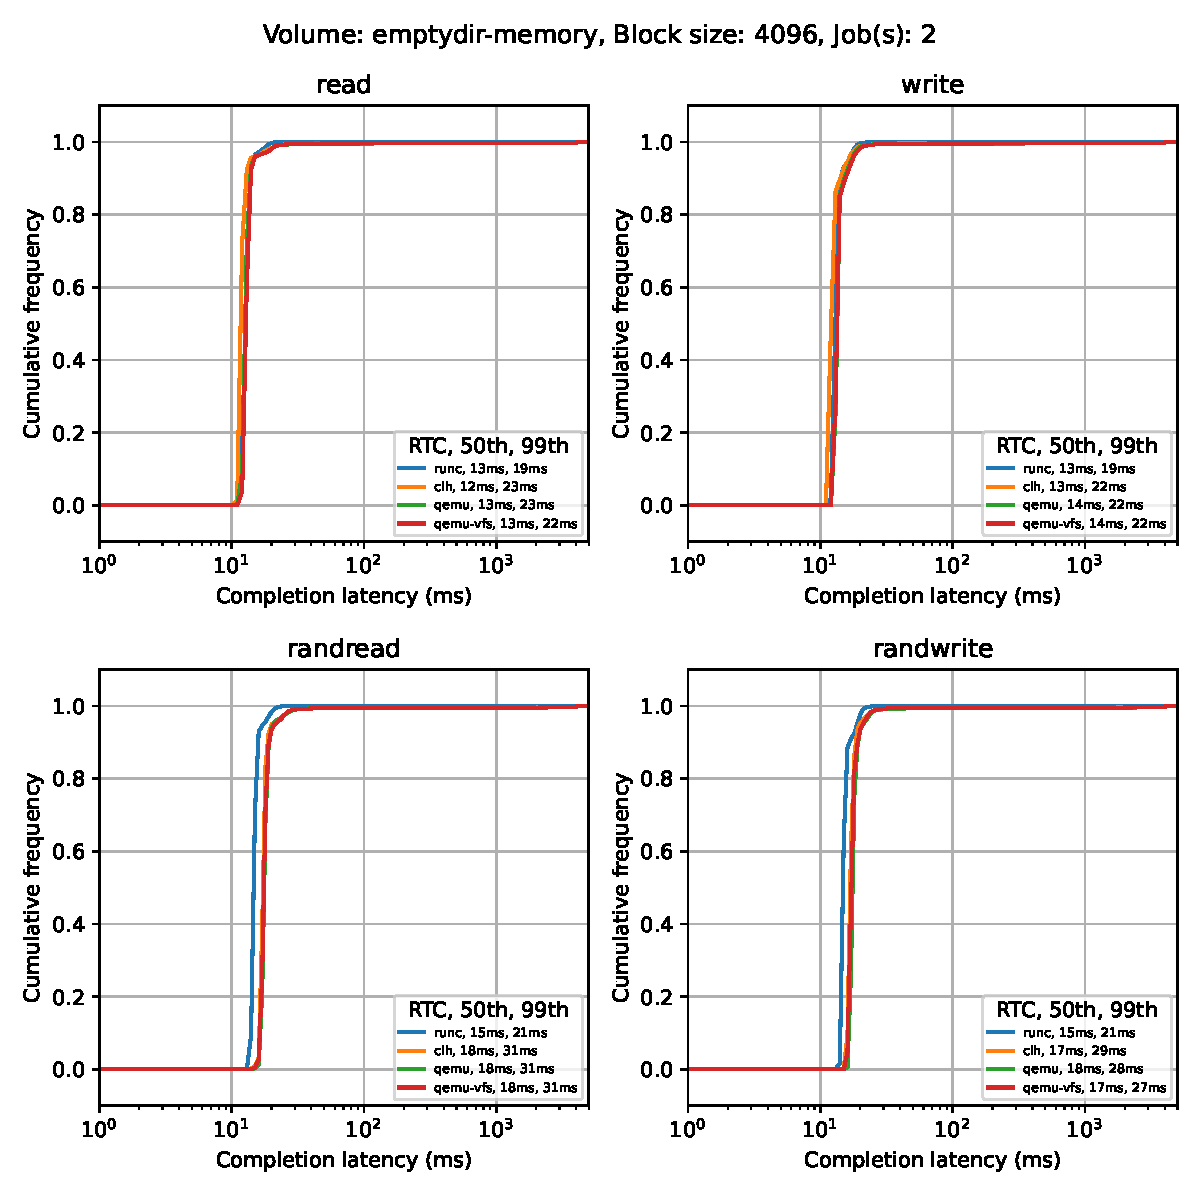
\includegraphics[width=12cm]{results/subplot_clat_bw_by_rw(emptydir-memory,2,4096).pdf}
    \caption{Completion latency for memory-based emptyDir by runtime classes for 4096 bytes block size and two jobs}
    \label{fig:ResultsEDMEMClatByRTC4096-2}
  \end{center}
\end{figure}

\begin{figure}[ht]
  \begin{center}    
    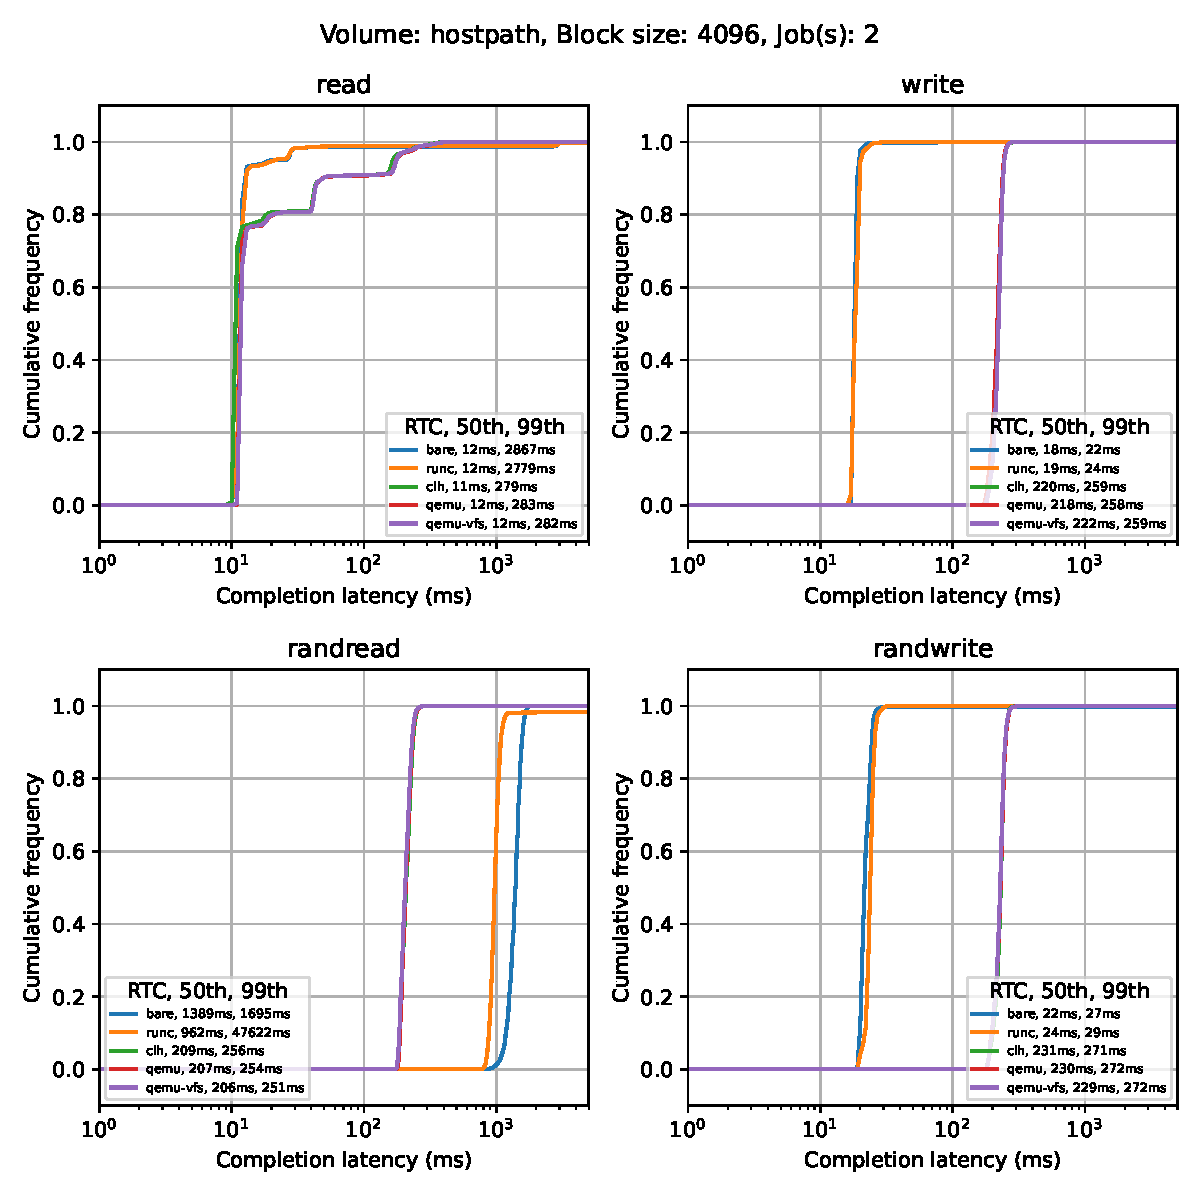
\includegraphics[width=12cm]{results/subplot_clat_bw_by_rw(hostpath,2,4096).pdf}
    \caption{Completion latency for hostPath by runtime classes for 4096 bytes block size and two jobs}
    \label{fig:ResultsHPClatByRTC4096-2}
  \end{center}
\end{figure}

\section{Evaluation}

Caching of the hypervisor significantly affects the received performance results and limits the absolute measurement of the micro-VM's overhead. However, some objections can be derived from the acquired results with confidence. Firstly, Kata Containers acquires close to runC's performance with memory-based emptyDir I/O operations with approximately an 8\% increase in completion latency for 4 kB block size. 

Kata Containers adds overhead to bandwidth and latency to task completion for disk-based operations. In these write operations, the bandwidth overhead is approximately 33-40\% in comparison to runC. For hostPath, the added latency averages around 250 ms even for the first percentile to complete. The architecture of Kata Containers includes a constant delay for the tasks, which stems from the data passing through more components, such as kata-agent and the hypervisor. In contrast, runC relies on a more simple environment allowing instant data transmission. A similar performance trend follows in other disk-based volumes.

The block size of the performance test also affects the results. For smaller block sizes between 512 and 8192, CLH outperforms QEMU-based runtime classes. However, the trend flips for the largest two block sizes in favor of QEMU and QEMU with VirtioFS.

%\textcolor{red}{Transition to Discussion missing?}